\documentclass[RNAAS]{aastex631}

% Numbers are \input from the pipeline-generated macros -- none typed by hand.
% Auto-generated by jansky_research.lvdrift.write_paper_macros -- do not edit.
\newcommand{\lvdriftSource}{real LV614 type III arrays}
\newcommand{\lvdriftRealNBursts}{290}
\newcommand{\lvdriftRealNPass}{43}
\newcommand{\lvdriftRealFracPass}{15}
\newcommand{\lvdriftRealMedA}{1.45}
\newcommand{\lvdriftRealAqLo}{0.26}
\newcommand{\lvdriftRealAqHi}{2.32}
\newcommand{\lvdriftRealRobLo}{1.42}
\newcommand{\lvdriftRealRobHi}{1.82}
\newcommand{\lvdriftRealRobIncl}{3}
\newcommand{\lvdriftRealRobN}{9}
\newcommand{\lvdriftRealJointA}{-0.26}
\newcommand{\lvdriftRealJointChi}{220}
\newcommand{\lvdriftSynPoneBias}{-0.11}
\newcommand{\lvdriftRealPoneWin}{217}
\newcommand{\lvdriftRealNoneRej}{100}
\newcommand{\lvdriftRealRzeroThree}{1.34}
\newcommand{\lvdriftRealRzeroOne}{1.72}
\newcommand{\lvdriftRealRzeroFive}{1.08}
\newcommand{\lvdriftRealRzeroN}{201}
\newcommand{\lvdriftRealAcross}{0.23}
\newcommand{\lvdriftRealSelPass}{47.7}
\newcommand{\lvdriftRealSelFail}{39.1}
\newcommand{\lvdriftRealDriftFortyFive}{6.8}


\newcommand{\code}[1]{\texttt{#1}}

\begin{document}

\title{No Constraint on the Type III Drift-Rate Index from the LV614 LOFAR Burst Catalogue}

\author[0009-0008-3289-4447]{Joseph Barbere}
\affiliation{Independent researcher}

\begin{abstract}
\citet{steinbergs2026} fit $df/dt=Af^{a}$ to type III solar radio bursts recorded at 29--60~MHz by
the LOFAR station LV614 and report $a=0.43\pm0.31$, an across-burst relation whose amplitude is
consistent with zero. We fitted the drift law within each of the \lvdriftRealNBursts\ released
type III dynamic spectra. Only \lvdriftRealNPass\ bursts (\lvdriftRealFracPass\%) give a usable
ridge; their indices have an interquartile range of \lvdriftRealAqLo--\lvdriftRealAqHi\ around a
median of \lvdriftRealMedA, and one shared index fits them with $\chi^2/\nu\approx$
\lvdriftRealJointChi. The catalogue does not constrain the drift-rate index.
\end{abstract}

\section{Data and method}
\label{sec:method}
The catalogue \citep{steinbergs2026} lists 335 bursts with one drift rate each, measured at the time
of peak flux, and fits the law across bursts in 1~MHz bins of peak frequency (their Section~III.5,
Figure~15). The dynamic spectra are public \citep{lv614data} at 1~s and 195~kHz resolution. Across
bursts the law cannot constrain the index well: the band spans only a factor of two in frequency.
We therefore fitted it along each burst. For $df/dt=-Af^{a}$ the arrival time at frequency $f$ is
$t(f)=t_0-g(f;a)/A$ with $g=(f^{1-a}-f_{\rm ref}^{1-a})/(1-a)$. We took the arrival time in each
channel as the peak of the smoothed spectrum, kept channels with a peak signal-to-noise ratio of at
least 5, and required at least 40 channels spanning a frequency ratio of 1.5 with arrival times
falling monotonically to within 2~s.

Bursts planted into the first 20~s of \lvdriftRealPoneWin\ real spectra, with indices from 0 to
1.84, were recovered to within 0.15, although a planted 1.23 was read low by \lvdriftSynPoneBias.
Spectra with their channels shuffled in time were rejected in \lvdriftRealNoneRej\% of cases.

\section{Results}
\label{sec:results}
The quality cut is passed by \lvdriftRealNPass\ of \lvdriftRealNBursts\ type III bursts; most of the
rest have a ridge that jumps to another burst or to interference in the same spectrum. The bursts
that pass peak at higher frequency than those that fail (medians \lvdriftRealSelPass\ and
\lvdriftRealSelFail~MHz), so the result describes bursts that stay coherent across the band. Their
fitted indices (Figure~\ref{fig:index}) scatter far more than the planted bursts, with an
interquartile range of \lvdriftRealAqLo--\lvdriftRealAqHi\ and a median of \lvdriftRealMedA. Over
nine combinations of signal-to-noise threshold and smoothing the median ranges from
\lvdriftRealRobLo\ to \lvdriftRealRobHi, and its 95\% interval contains the index of 1.23 found at
10--80~MHz by \citet{zhang2018} in \lvdriftRealRobIncl\ of the \lvdriftRealRobN\ cases. A single
index shared by all passing bursts fits with $\chi^2/\nu\approx$ \lvdriftRealJointChi\ for a 1~s
timing error, so no one law describes them at this resolution.

Re-fitting the catalogue's own drift rates without binning gives $a=$ \lvdriftRealAcross, within
the published uncertainty. Our drift at peak flux exceeds the catalogue value by a median factor of
\lvdriftRealRzeroThree\ for a $\pm3$~s regression window and of \lvdriftRealRzeroFive\ for $\pm5$~s
(\lvdriftRealRzeroN\ bursts); the catalogue does not state its window.

\section{Conclusion}
\label{sec:conclusion}
At 29--60~MHz and 1~s resolution these spectra do not constrain the drift-rate index: the
across-burst value is consistent with zero amplitude, and the within-burst indices are broader than
the method's resolution and are not described by a single law. A within-burst index is a different
quantity from the across-burst value and the two are not in tension. The drift laws of
\citet{alvarez1973} and \citet{zhang2018}, derived over wider bands, remain the reference.

\begin{figure}[ht]
\centering
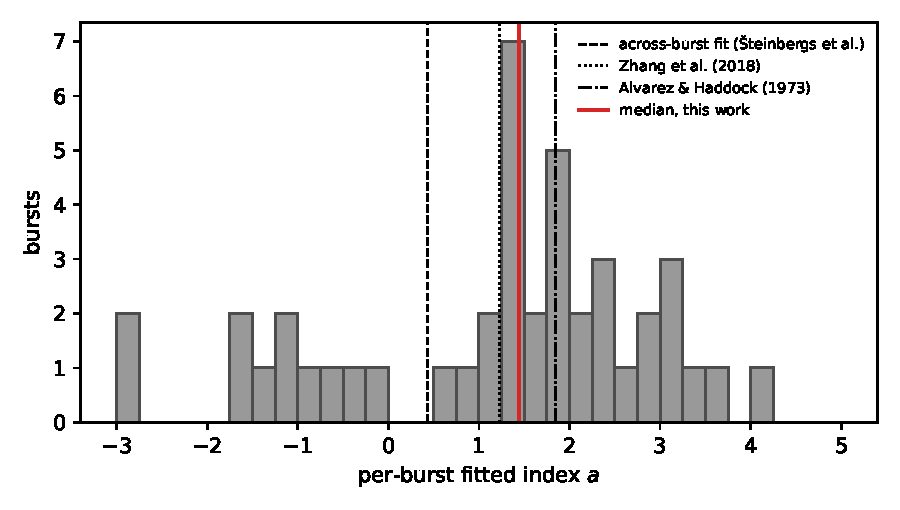
\includegraphics[width=\linewidth]{figures/lvdrift_index.pdf}
\caption{Fitted drift-rate indices of the \lvdriftRealNPass\ LV614 type III bursts that pass the
quality cut, with the catalogue's across-burst fit, the index of \citet{zhang2018} and that of
\citet{alvarez1973}.}
\label{fig:index}
\end{figure}

\software{\code{jansky-research} \citep{janskyresearch}, \code{jansky} \citep{jansky}, NumPy, SciPy,
Matplotlib. Analysis assisted by Claude \citep{anthropicclaude}. The estimator and its controls are
covered by an offline test suite; the data drivers are not unit-tested.}

\bibliography{refs}
\bibliographystyle{aasjournal}

\end{document}
